\documentclass[a4paper,12pt]{report}                % Format standard pour les mémoires
\usepackage{packages, macros}                       % Chargement des packages et macros

\begin{document}
% Page de garde
\begin{titlepage}
    \newgeometry{top=0cm, bottom=0cm, left=1.5cm, right=0.5cm} % Marges spécifiques à la page de garde
    \begin{tikzpicture}[remember picture, overlay]
        \fill[bleufonce] ([xshift=1cm]current page.north west) rectangle ([xshift=2cm,yshift=-6cm]current page.north west); % Rectangle en haut à gauche
        \fill[blue] (current page.north east) -- ([xshift=-1cm]current page.north east) -- ([yshift=-10cm]current page.north east) -- cycle; % Triangle en haut à droite
        \fill[blue] ([xshift=1cm] current page.south west) rectangle ([xshift=2cm,yshift=11cm]current page.south west); % Rectangle en bas à gauche
        \fill[bleufonce] (current page.south east) -- ([xshift=-1cm]current page.south east) -- ([yshift=10cm]current page.south east) -- cycle; % Triangle en bas à droite
    \end{tikzpicture}
    \begin{center}
        \begin{minipage}{0.92\textwidth}
            
\includegraphics[width=7cm]{images/logo_fst_1.png}
            \hfill
            
\includegraphics[width=3cm]{images/logo_ubs.png}
        \end{minipage}\\[0.1cm]
        
\includegraphics[width=6cm]{images/logo_campus.png}\\[1cm]
        \HRule \\[0.5cm]
        \textcolor{bleufonce}{\textbf{\textsc{\LARGE Mémoire de Recherche de II CYCLE}}} \\[1.5cm]
        \begin{tcolorbox}[
            enhanced,                   % active les fonctionnalités avancées
            colback=blue,
            colframe=blue,
            arc=3mm,
            boxrule=0mm,
            width=18cm,
            fontupper=\color{white}, 
            center title, 
            drop shadow={black!50!white, shadow xshift=2.5pt, shadow yshift=--2pt,opacity=0.6}
            ]
            \centering
            \textbf{\LARGE Analyse de l'impact des récentes réformes du baccalauréat au Sénégal sur le taux de réussite au bac et le parcours universitaire des bacheliers}
        \end{tcolorbox}
        \vspace{1.5cm}
        \textbf{\textit{\large Présenté et soutenu par:}}\\[0.5cm]
        \textcolor{blue}{\textbf{\LARGE ABDOUROIHIM Attoumane}}
    \end{center}
    \vspace{1cm}
    \begin{flushleft}
        \hspace{0.5cm} 
        \textmd{\large Pour l'obtention du double diplôme de \textbf{\Large Master 2},}
        \begin{center}
            \textmd{\Large \textcolor{blue}{\textbf{D'Ingénierie Mathématique et Numérique}}}
        \end{center}
        \vspace{0.5cm}
        \hspace{0.5cm}
        \textmd{\large Sous la direction de : \textbf{\Large Pr Bamba GUEYE \& Pr Mountaga LAM}}\\  
        \vspace{1cm}
        \hspace{1cm}
        \textit{\large Présenté le 5 juillet 2025, devant le jury composé de :}\\
        \vspace{0.5cm}
        \begin{center}
        \hspace{3cm}
        \begin{minipage}{0.3\textwidth}
            \textmd{\Large Dr Souley KANE }\\[0.3cm]
            \textmd{\Large Pr Papa NGOM}\\[0.3cm]
            \textmd{\Large Dr Boubacar DIAO}
        \end{minipage}
        \hfill
        \begin{minipage}{0.4\textwidth}
            \textmd{\large Maître de conférence}\\[0.3cm]
            \textmd{\large Professuer Titulaire (President)}\\[0.3cm]
            \textmd{\large Maître de conférence}
        \end{minipage}
    \end{center}
    \end{flushleft}
    
\end{titlepage}
    \restoregeometry % Restauration des marges globales
    % Dédicace
    \begin{center}
        \section*{\textsc{\LARGE Dédicace}}
    \end{center}
    \bigskip
    \textbf{Je dédie ce travail à ma famille :}

    \bigskip

    À mes parents, M. \textbf{ATTOUMANE Abdallah} et Mme \textbf{ZALIHATAH Abdallah}, qui ont été un soutien inconditionnel tout au long de mon parcours académique, 
    tant sur le plan financier que moral. Merci pour vos conseils dans mes moments de doute et pour votre présence constante dans tous mes choix et dans toute ma vie.

    \bigskip

    À ma femme, Mme \textbf{ADELIA Soiffaouiddine}, dont la présence à mes côtés a été essentielle pour affronter cette vie ensemble. 
    Sans elle, ce travail n’aurait tout simplement pas existé.

    \bigskip

    À mes deux grandes sœurs, Mme \textbf{ITFAOU Attoumane} et Mme \textbf{ROIHMA Attoumane}, pour leur affection et leur soutien inconditionnel.

    \bigskip

    À ma belle-famille, en particulier Dr \textbf{SOIFFAOUIDDINE Sidi}, le père de ma femme, pour son aide précieuse, tant financière que morale, 
    et pour la confiance qu’il m’a accordée en acceptant de me donner sa fille la plus précieuse.
    % Remerciements
    \newpage
    \begin{center}
        \section*{\textsc{\LARGE Remerciements}}
    \end{center}
    \bigskip
    \textbf{\large Alhamdulillah Rabbi al-‘Alamin.}

    \medskip

    Ya \textbf{\textsc{\Large Allah}}, merci de m'avoir permis de réaliser ce travail, de m'avoir donné la force et le courage d'affronter toutes les difficultés que j'ai pu rencontrer.

    Je tiens à témoigner toute ma reconnaissance et mes remerciements les plus sincères au \textbf{\large Professeur Mountaga LAM}, mon directeur à la DES et encadrant professionnel de ce travail.

    Merci, tout d’abord, de m’avoir permis d’obtenir mon tout premier travail professionnel et salaire de ma vie en m’acceptant pour travailler sous votre direction à la DES. Merci pour votre patience, vos encouragements, 
    votre disponibilité, votre confiance et vos nombreux conseils précieux.\\
    \textit{ C’est un immense honneur d’avoir pu travailler avec vous.}

    Je remercie également le \textbf{Professeur Bamba GUEYE}, directeur de l’Office du Bac et encadrant académique de ce travail, pour ce sujet particulièrement stimulant, pour sa disponibilité et ses conseils précieux tout au long de ce travail.

    Je tiens à remercier tout particulièrement \textbf{Dr Souley KANE}, mon directeur de formation, qui m’a permis d’obtenir ce stage et qui a profondément changé ma vie professionnelle en m’ouvrant les portes d’un monde d’opportunités que je n’aurais jamais imaginé intégrer.

    Je n’oublierai pas mes collègues à la DES, en particulier Madame \textbf{MBAYE} et Madame \textbf{PAYE} qui, par leur hospitalité et leur gentillesse, ont été comme des mères pour moi.
    Merci à vous et ainsi qu’à tous mes autres collègues de travail pour votre aide précieuse tout au long de mon stage.

    Je remercie également \textbf{les membres du jury} pour l’attention accordée à ce travail, ainsi que pour leurs remarques pertinentes et enrichissantes.

    Je remercie tous \textbf{les camarades} que j’ai rencontrés au fil de mon parcours pour leur fraternité et leur présence.

    Ma profonde gratitude va à l’endroit de tous \textbf{les enseignants} qui m’ont transmis leur savoir avec passion.Grâce à vous, je suis devenu la personne que je suis aujourd’hui.

    \vspace{0.5cm}
    \hfill \textit{Merci infiniment à tous, c'était un honneur.}

    % Résumé et Abstract
    \newpage
    \section*{\textsc{Résumé}}

    Ce mémoire de recherche, intitulé "Analyse de l'impact des récentes réformes du baccalauréat au Sénégal sur le taux de réussite au bac et le parcours universitaire des bacheliers", étudie les effets des modifications structurelles du baccalauréat sénégalais entre 2006 et 2024. 
    L'analyse se décompose en deux axes majeurs : l'évolution du taux de réussite au baccalauréat par série et la trajectoire des bacheliers à l'Université Cheikh Anta Diop (UCAD).

    Nos résultats montrent une stabilisation des effectifs au bac après une forte croissance, et un rebond du taux de réussite global après une période de déclin. 
    Les réformes ont eu un impact notable sur les séries spécifiques : la transition de la série G vers la STEG est un succès quantitatif et qualitatif, avec des taux de réussite nettement améliorés. 
    De même, la série Littératures et Civilisations Arabes (L-AR) a connu une croissance fulgurante de ses effectifs tout en maintenant des performances solides, démontrant une meilleure structuration des filières arabes. 
    La série Sciences Appliquées (S2A) gagne en attractivité et en réussite. 
    En revanche, la série Sciences Fondamentales (S1A) reste marginale malgré un taux de réussite très élevé, et l'implémentation de certaines filières scientifiques arabes reste incomplète.
    
    Concernant le parcours universitaire à l'UCAD, les bacheliers STEG et G s'orientent majoritairement vers la FASEG et les départements de gestion. 
    Les bacheliers des séries arabes (LA et LAR) se dirigent principalement vers la FLSH et le département d'Arabe. Les bacheliers scientifiques (S2A et S1A) intègrent la FST, avec des ouvertures vers la FASEG et la FMPO pour la S2A. 
    Ces observations confirment une cohérence entre les nouvelles orientations du baccalauréat et les filières universitaires choisies.

    \newpage
    \section*{\textsc{Abstract}}

    This research thesis, titled "Analysis of the impact of recent baccalaureate reforms in Senegal on baccalaureate success rates and graduates' university pathways," investigates the effects of structural changes to the Senegalese baccalaureate between 2006 and 2024. 
    The analysis is divided into two main areas: the evolution of baccalaureate success rates by series and the trajectory of graduates at Cheikh Anta Diop University (UCAD).
    
    Our findings indicate a stabilization of baccalaureate enrollment after a period of rapid growth, and a rebound in the overall success rate following a period of decline. 
    The reforms have had a significant impact on specific series: the transition from the G series to the STEG series is a quantitative and qualitative success, with significantly improved success rates. Similarly, the Arabic Literature and Civilizations (L-AR) series has seen explosive growth in enrollment while maintaining solid performance, demonstrating better structuring of Arabic-language programs. 
    The Applied Sciences (S2A) series is gaining attractiveness and success. 
    Conversely, the Fundamental Sciences (S1A) series remains marginal despite a very high success rate, and the implementation of certain Arabic scientific programs remains incomplete.

    Regarding university pathways at UCAD, STEG and G graduates primarily orient themselves towards FASEG and management departments. Graduates from Arabic series (LA and LAR) mainly head to FLSH and the Arabic department. 
    Science graduates (S2A and S1A) enter FST, with openings towards FASEG and FMPO for S2A. 
    These observations confirm a coherence between the new baccalaureate orientations and the chosen university programs.

    % Table des matières
    \newpage
    \tableofcontents


    % Table des figures 
    \newpage
    \listoffigures

    % Liste des codes
    % \newpage
    \lstlistoflistings
    
    % Liste des tableaux
    % \newpage
    \listoftables
    

    % Importation des chapitres

    \chapter*{Introduction Générale}
\markboth{\large Introduction Générale}{}
\addcontentsline{toc}{chapter}{Introduction Générale}

\section*{Contexte et justification}
\addcontentsline{toc}{section}{Contexte et justification}

Le système éducatif sénégalais, hérité du modèle français, repose sur une structuration en trois cycles : primaire, moyen et secondaire. 
La fin du secondaire est sanctionnée par le baccalauréat, diplôme pivot marquant l'accès à l'enseignement supérieur et considéré comme le premier grade universitaire. 
Il joue un rôle central, non seulement en tant que certificat de fin d’études, mais aussi comme indicateur de performance du système éducatif.

Malgré les réformes successives visant à adapter ce diplôme aux réalités nationales et aux enjeux contemporains, le baccalauréat au Sénégal reste confronté à un taux de réussite relativement faible, 
oscillant autour de 40\%, loin des standards observés dans des pays comme la France ou le Canada où il s'oscille au tour de 99\% \cite{Mbaye2023}. 
Ce paradoxe entre le nombre croissant de candidats et la stagnation du taux de réussite interroge sur l’efficacité des politiques éducatives mises en œuvre.

Dans ce contexte, plusieurs réformes majeures ont été introduites : l’instauration du baccalauréat arabo-français en 2000, la création du bac arabe en 2013, 
et la transformation de la série G en série STEG (Sciences et Techniques de la Gestion) en 2019. 
Ces réformes traduisent la volonté des autorités d’élargir les opportunités d’accès à l’enseignement supérieur, de diversifier les profils de bacheliers, 
et d'améliorer l'adéquation entre formation et marché du travail. Ce mémoire se propose d’évaluer l’impact réel de ces transformations sur le taux de réussite au baccalauréat et sur le parcours universitaire des bacheliers, notamment à l'UCAD.

\section*{Problématique et Objectifs de l'étude}
\addcontentsline{toc}{section}{Problématique et Objectifs de l'étude}

Les réformes successives du baccalauréat sénégalais, notamment l’introduction du bac arabe en 2013 et de la série STEG en 2019,
ont été motivées par la volonté de moderniser le système éducatif, de mieux adapter l’offre de formation aux besoins socio-économiques du pays et de favoriser l’inclusion. 
Toutefois, leur impact réel reste encore peu documenté de manière rigoureuse.

Une question centrale se pose :

\textbf{Ces réformes ont-elles réellement contribué à améliorer les performances au baccalauréat et à faciliter le parcours universitaire des nouveaux bacheliers ?}

Plusieurs interrogations découlent de cette problématique :
\begin{itemize}
    \item Les réformes ont-elles eu un effet mesurable sur les taux de réussite au baccalauréat, globalement et par série ?
    \item Comment les nouvelles séries, comme le bac arabe ou la série STEG, se positionnent-elles en termes de performances au bac ?
    \item Comment les bacheliers issus des séries arabes évoluent-ils dans l’enseignement supérieur, notamment à l’UCAD ?
    \item Existe-t-il des disparités significatives entre les différentes séries du baccalauréat en termes de réussite et d’insertion à l'UCAD ?
\end{itemize}

À travers une analyse des données du baccalauréat (2006–2024) et des inscriptions à l’UCAD (2002–2024), ce travail poursuit plusieurs objectifs :
\begin{itemize}
    \item \textbf{Analyser l’évolution des taux de réussite au bac}, avec une attention particulière aux périodes post-réformes.
    \item \textbf{Modéliser et prédire les taux de réussite} pour estimer ce qu’ils auraient été sans réformes (approche contrefactuelle).
    \item \textbf{Étudier le parcours universitaire des bacheliers (suivi de cohortes)}, en identifiant les départements, filières et performances selon les séries d’origine.
    \item Fournir des \textbf{recommandations basées sur les données} pour orienter les politiques éducatives futures.
\end{itemize}

Ce travail vise ainsi à combler un manque crucial d’évaluation quantitative des réformes éducatives,
en mobilisant des méthodes statistiques, des modèles prédictifs et des visualisations, pour offrir une lecture factuelle et visuelle des effets des réformes, afin d’éclairer la prise de décision dans le secteur éducatif.

\section*{Méthodologie et Organisation du document}
\addcontentsline{toc}{section}{Méthodologie et Organisation du document}

Cette étude repose sur une démarche méthodologique structurée, combinant analyse statistique, modélisation prédictive et visualisation avancée. L’objectif est d’évaluer de manière quantitative et visuelle l’impact des réformes du baccalauréat sur la réussite scolaire et le parcours universitaire.
\newpage
La méthodologie adoptée comprend :

\begin{itemize}
    \item Une \textbf{revue des réformes éducatives} ayant marqué le baccalauréat sénégalais.
    \item L’exploitation de trois grandes bases de données : les \textbf{résultats du baccalauréat} (2006–2024), les \textbf{inscriptions universitaires à l’UCAD} (2002–2024) et les \textbf{résultats universitaires à l’UCAD} (2011–2024).
    \item Une \textbf{analyse descriptive et prédictive}, appuyée par des représentations visuelles riches afin de faciliter la compréhension et l’interprétation des résultats.
    \item Un \textbf{suivi longitudinal des cohortes} de bacheliers à l’université, avec une attention particulière portée aux différences selon les séries d’origine.
    \item Une \textbf{restitution interactive} à l’aide de tableaux de bord dynamiques réalisés avec Power BI.
\end{itemize}


Le document est organisé en six chapitres principaux, suivis d'une section dédiée à la conclusion et aux recommandations, suivant la logique de cette démarche :

\begin{enumerate}
    \item \textbf{État de l’art} : Présentation des réformes du baccalauréat et revue des études antérieures sur le sujet.
    \item \textbf{Données et outils utilisés} : Description des sources de données et des outils mobilisés.
    \item \textbf{Nettoyage et préparation des données} : Traitement, fusion et structuration des données pour les rendre exploitables.
    \item \textbf{Analyse du taux de réussite au bac} : lecture visuelle et modélisation des taux avec simulations.
    \item \textbf{Analyse du parcours universitaire et suivi de cohortes} : visualisation du cheminement des bacheliers à l’UCAD.
    \item \textbf{Restitution interactive et visualisation} : Présentation des dashboard Power BI, incluant les filtres dynamiques, mesures, colonnes conditionnelles et visualisations interactives.
\end{enumerate}

\textbf{Conclusion et recommandations} : Bilan général de l’étude, limites rencontrées et propositions pour renforcer l’efficacité des politiques éducatives. % Importation de l'introduction générale

    \chapter{État de l’art}

\section{Introduction}

Depuis sa création, comme énoncé précédemment, le baccalauréat sénégalais a connu de nombreuses évolutions, tant dans sa structure que dans ses objectifs. 
Initialement conçu comme un simple diplôme de fin d’études secondaires, il est aujourd’hui devenu un véritable levier d’accès à l’enseignement supérieur et un indicateur clé de performance du système éducatif national.

Ce chapitre propose une revue synthétique des principales réformes ayant marqué l’histoire du baccalauréat au Sénégal, notamment celles de 1995, 2000, 2013 (introduction du bac arabe) et 2019 (création de la série STEG). 
Il s’agira d’examiner le contexte de leur mise en œuvre, les motivations qui les ont justifiées, ainsi que leurs ambitions en termes de modernisation, d’inclusion et de diversification des profils d’élèves.

Cette mise en perspective historique permet de mieux situer l’organisation de notre étude, qui vise à évaluer l’impact réel de ces réformes sur les performances scolaires (taux de réussite) et les parcours universitaires (suivi de cohortes à l’UCAD). 
Elle constitue ainsi une étape essentielle pour comprendre les enjeux de notre analyse et justifier le recours à une approche fondée sur les données et la visualisation interactive. 

\section{Historique et rôle du baccalauréat}

Le baccalauréat a été inventé en France au XIX\textsuperscript{e} siècle par un décret de l'empereur Napoléon Ier en 1808.
À l’origine appelé le \textbf{«~Bachot~»}, il tire son étymologie du latin médiéval \textit{ "bacca laurea"}, il désigne en latin médiéval \textbf{la couronne de laurier} remise aux vainqueurs \cite{bacHistorique}.

Dans le contexte sénégalais, il a été progressivement intégré au système éducatif colonial, puis nationalisé après l’indépendance. 
Il sanctionne la fin du cycle secondaire et donne accès à l’université, devenant ainsi un indicateur majeur de performance du système éducatif.

Aujourd’hui, le baccalauréat incarne à la fois une étape symbolique vers l’âge adulte et un enjeu stratégique pour le développement du capital humain, d’où l’importance des réformes visant à le rendre plus inclusif et mieux adapté aux réalités sociales et économiques du pays.

\section{Organisation du baccalauréat : structure et acteurs}

Le baccalauréat Sénégalais est organisé par \textbf{l'Office du baccalauréat}, rattaché à l'Université Cheikh Anta Diop de Dakar (UCAD), ce qui renforce l'idée qu'il constitue le premier diplôme universitaire.
Chaque année, son organisation mobilise plusieurs milliers d’acteurs : enseignants, surveillants, correcteurs et présidents de jury.

L’examen est structuré autour de différentes séries, réparties en trois grandes filières : \textbf{littéraire}, \textbf{scientifique} et \textbf{tertiaire}. 
Cette diversification vise à mieux prendre en compte la pluralité des profils et des parcours de formation des élèves. Les épreuves s’appuient sur des programmes nationaux fixés par le ministère de l'Éducation, et sont organisées de manière centralisée, tant dans leur déroulement que dans leur correction.

Ce travail est réalisé en étroite collaboration avec l’Office du Baccalauréat, ce qui permet un accès privilégié à certaines données et une meilleure compréhension des mécanismes internes liés à l’organisation et à l’évolution de l’examen.

\section{Réformes du baccalauréat au Sénégal}

Depuis les années 1990, plusieurs réformes ont été introduites pour adapter le baccalauréat aux réalités sociolinguistiques, 
économiques et pédagogiques du pays.

\subsection{Réformes de 1995 (décret n° 95-947)}

Certainement la réforme la plus marquante, elle s'inscrit dans le cadre de la concertation nationale sur l'enseignement supérieur tenu le 9 décembre 1995, 
dont sont issues les propositions de la commission qui avait été chargée de réfléchir sur l'examen du baccalauréat \cite{decret95}.

Elle a introduit les changements majeurs dans la structure des séries telles qu'on les connaît aujourd'hui, 
notamment par l'article 7 du décret établissant les choix des séries que les candidats devront choisir au moment de leurs inscriptions :

\begin{itemize}
    \item Série L1 : Langues et Civilisations
    \item Série L2 : Sciences sociales et humaines
    \item Série G : Techniques quantitatives d'économie et de gestion
    \item Série S1 : Sciences exactes (Mathématiques et Physique)
    \item Série S2 : Sciences expérimentales
    \item Série S3 : Sciences et Techniques
    \item Série T1 : Fabrication mécanique
    \item Série T2 : Électrotechnique-Électronique
\end{itemize}

C'est pour modifier et compléter cette article 7 du décret n°1995-947 que toutes les réformes étudiées dans ce mémoire ont été introduites.

\subsection{Réformes de 2000 (décret n° 2000-585)}

Apparue très tôt dans l'élémentaire, la langue arabe sera reconnue comme langue vivante étrangère au Sénégal, laissée au choix de l'élève dans l'enseignement moyen, puis secondaire.

Parallèlement à cette évolution dans l'enseignement public, l'initiative privée, portée par une demande socio-culturelle, a donné naissance à un système d'enseignement arabe encore embryonnaire.
Ainsi, avec la multiplication des établissements exclusivement arabe ou bilingue franco-arabe, la nécessité d'encadrer ce phénomène a conduit l'État sénégalais à mettre en place un référentiel de diplôme : 
c'est la création du \textbf{Certificat arabe} et du \textbf{BFEM arabe} \cite{decret2000}.

La création du collège public franco-arabe \textbf{Mouhamadou Fadilou Mbacké} de Dakar en 1963 procéde de cette volonté de répondre à cette demande sociale. Un second cycle y a été mis en place, offrant les même perspectives que celles proposées aux autres collégiens.
Ainsi, le décret n°2000-585 du 6 juillet 2000 a introduit le baccalauréat option arabe qui modifie l'article 7 du décret n° 95-947 en un article 7 bis en intégrant les baccalauréats option arabe suivants : 

\begin{itemize}
    \item Langues et Sciences sociales : LA
    \item Sciences fondamentales : S1A
    \item Sciences appliquées : S2A
\end{itemize}

\subsection{Réformes de 2013 (décret n° 2013-913)}

\textit{"Le baccalauréat organisé (matérialisé) par le décret n°2000-586 du 20 juillet 2000, 
n'a pas atteint tous ses objectifs car des écoles privées franco-arabes et des instituts islamiques se multiplient entraînant un manque de contrôle
sur les programmes enseignés ainsi qu'une prolifération de diplômes qui empêche l'existence d'un standard commun à toutes les études secondaires du pays"}\cite{decret2013}.

C'est pour encadrer ce phénomène que, tout comme les études secondaires franco-arabes, les études secondaires arabes seront sanctionnées par les baccalauréats arabes. 
Ces derniers sont définis dans un article 7 ter, qui complète l'article 7 bis du décret n° 2000-585, en intégrant les séries suivantes :

\begin{itemize}
    \item Littératures et Civilisations arabes : L-AR 
    \item Mathématiques et Sciences Physique : S1-AR
    \item Sciences expérimentales : S2-AR
\end{itemize} 

\textbf{Remarque importante :}
Il convient de souligner que, bien que le décret n° 2013-913 ait introduit les séries \textbf{S1-AR} et \textbf{S2-AR},
les données disponibles et la pratique sur le terrain indiquent que ces séries scientifiques n'ont \textbf{jamais été concrètement mises en place ni organisées} depuis la promulgation de ce décret.
Seule la série L-AR est actuellement opérationnelle.

\subsection{Réformes de 2019(décret n° 2019-645)}

À la difference des précédentes réformes, celle-ci à pour but de renforcer la série G aux exigences des Formations Professionnelles et Techniques(FPT)
et des Instituts Supérieurs d'Enseignement Professionnel (ISEP).

\textit{"C'est dans ce cadre qu'il est proposé que la série G (économie et gestion) soit transformée en série technologique (sciences et technologique de l'économie et de la gestion : STEG)
visant essentiellement à installer chez les élèves les compétences en associant la culture générale et la technologie"}\cite{decret2019}.

\section{Travaux antérieures }

Plusieurs études ont porté sur la performance du système éducatif sénégalais et l’évolution du baccalauréat.

L’article de Diagne (2023) analyse l’évolution du taux de réussite au bac sur deux décennies (2001–2022). 
Il met en évidence l’instabilité chronique du système, marquée par une réussite oscillant autour de 40\%, bien inférieure aux standards internationaux. 
L’auteur identifie plusieurs facteurs influents : interruptions pédagogiques, surcharge des programmes, conditions socio-économiques, etc. 
Malgré les nombreuses réformes (EPT 1990, PDEF 2003, PAQUET-ET 2013), les performances restent en deçà des attentes \cite{Mbaye2023}.

Par ailleurs, le rapport de la DES de l’UCAD (2021) adopte une approche longitudinale de suivi de cohorte pour évaluer l’efficacité interne des formations universitaires. 
À partir de la cohorte 2013-2014, il retrace les parcours des étudiants selon leur série de bac et leur établissement d’accueil à l’UCAD. 
Cette étude montre des taux importants de redoublement et d’abandon dès les premières années universitaires, avec des écarts marqués selon les séries d’origine \cite{des2021}.

Ces travaux révèlent un manque d’articulation entre les réformes du bac et les trajectoires universitaires, d’où l’importance d’une évaluation intégrée comme celle proposée ici.

\section{Approche méthodologique et innovante de l'étude}

Ce travail s’inscrit dans le cadre d’un stage à la Direction des Études et des Statistiques (DES) de l’UCAD, en collaboration avec l’Office du Baccalauréat. 
Il combine une analyse data-driven et exploratoire de données pour évaluer l’impact des réformes sur deux axes :
\begin{enumerate}
    \item \textbf{performance académique}: Analyse de l'évolution du taux de réussite au bac de 2006 à 2024 globale et des séries concernées.
    \item \textbf{performance universitaire}: Une suivi des cohortes ici des séries concernées du bac, avec une attention particulière à leur insertion et leur progression à l’UCAD. 
\end{enumerate}
Un \textbf{tableau de bord interactif} sera mis en place pour visualiser les résultats de l'analyse et permettre une exploration dynamique des données, en vue de faciliter la prise de décision et la formulation de recommandations éclairées.

\section{Conclusion}

Ce premier chapitre a permis de retracer l’évolution historique et structurelle du baccalauréat au Sénégal, en mettant en évidence les principales réformes qui l’ont façonné depuis les années 1990. 
Motivées par des enjeux pédagogiques, socioculturels et économiques, ces réformes ont conduit à une transformation en profondeur du système : modification des séries existantes, introduction de nouvelles séries, et adaptation progressive aux réalités nationales.
 % Importation du chapitre 1

    \chapter{Données et outils utilisés}

\section{Introduction}

Ce chapitre introduit les données exploitées ainsi que les outils utilisés pour mener à bien notre analyse. 
Il constitue une étape essentielle dans la construction de l’étude, car la qualité et la structuration des données conditionnent la pertinence des résultats.

Les données utilisées couvrent une période suffisamment large pour permettre des comparaisons temporelles et une évaluation rigoureuse des effets des réformes. 
Elles ont été préparées et organisées en vue de faciliter les analyses statistiques, les visualisations, ainsi que les modélisations prédictives.

Les outils mobilisés permettent à la fois le traitement, l’analyse et la visuelle claire et dynamique des résultats. 

\section{Sources et Description des données}

\subsection{Sources de données}

Ce projet s’appuie sur trois principales sources de données fournies par deux institutions officielles : 
\begin{itemize}
    \item \textbf{l’Office du Baccalauréat du Sénégal}, chargé de l’organisation de l’examen et de la production des résultats officiels du bac sur l’ensemble du territoire national ;
    \item \textbf{la Direction de l’Informatique et des Systèmes d’Information (DISI)} de l’UCAD, responsable de la gestion des données académiques et administratives à l’université ;
\end{itemize}

\subsection{Description des données}


L’étude repose sur trois ensembles de données complémentaires, couvrant le parcours des apprenants depuis l’obtention du baccalauréat jusqu’à leur progression dans l’enseignement supérieur à l’UCAD.

\subsubsection{Résultats du Baccalauréat (2006--2024)}

Ces données ont été fournies par l’Office du Baccalauréat du Sénégal. 
Elles contiennent les informations relatives aux candidats (année, série, résultat, mention, session, etc.). 
Elles permettent de mesurer les taux de réussite globaux et par série, et de suivre l’impact des réformes.

\subsubsection{Inscriptions universitaires à l’UCAD (2002--2024)}

Issues de la Direction de la DISI, ces données renseignent sur le profil des étudiants inscrits à l’UCAD : année d’inscription, série d’origine au bac, établissement d’accueil, etc. 
Elles offrent une vision globale de l’évolution des flux d’entrée à l’université selon les caractéristiques des bacheliers.

\subsubsection{Résultats académiques à l’UCAD (2010--2024)}

Ces données, également fournies par la DISI, détaillent la performance universitaire des étudiants : moyennes annuelles, crédits, session, mention, résultats. 
Elles permettent d’apprécier la réussite dans le supérieur en fonction du parcours scolaire initial.

\bigskip

La combinaison de ces trois bases~--~résultats au bac, inscriptions et performances universitaires~--~permet de reconstruire des trajectoires individuelles et de réaliser un suivi de cohorte. 
Grâce aux variables communes (année, série du bac, résultat, etc.), il est possible de lier le profil d’entrée des étudiants à leur évolution à l’université, et d’évaluer ainsi l’impact des séries du baccalauréat sur leur réussite postscolaire.

\section{Outils et Technologies utilisés}

\subsection{Python et ses bibliothèques }


\includegraphics[width=3cm]{images/python.png}

Python est un langage de programmation open source, interprété, 
simple à apprendre et largement utilisé dans le domaine scientifique et technique.
Python s’est imposé comme l’un des outils les plus puissants pour l’analyse de données et le développement de modèles d’intelligence artificielle, 
notamment en raison de la richesse de ses bibliothèques spécialisées \cite{python}.

Dans le cadre de cette étude, Python a été utilisé à la fois pour le traitement, l’exploration et la visualisation des données,
ainsi que pour le développement de modèles de machine learning.

\subsubsection{bibliothèques utilisées}


\includegraphics[width=3cm]{images/Pandas_logo.png}

Pandas est une bibliothèque Python spécialisée dans la manipulation et l’analyse de données. 
Elle offre des structures de données flexibles et efficaces, notamment les \textbf{DataFrame}, 
qui permettent de gérer facilement des tableaux de données similaires à ceux d'Excel ou d'une base de données\cite{pandas}.

C’est sans doute le package le plus utilisé en science des données. Grâce à ses nombreuses fonctionnalités,
il ma permet de charger, filtrer, nettoyer et transformer les jeux de données de manière rapide et intuitive.


\includegraphics[width=4cm]{images/Matplotlib.png}

Matplotlib est une bibliothèque Python dédiée à la visualisation de données. 
Elle permet de créer une grande variété de graphiques statiques. 
Son interface simple et sa compatibilité avec les structures de données 
comme les DataFrame de pandas en font un outil de choix pour représenter visuellement les résultats d’une analyse \cite{matplotlib}.

\newpage

\includegraphics[width=3cm]{images/sckitlearn.png}

Scikit-learn est une bibliothèque Python dédiée au machine learning. 
Elle offre des outils simples et efficaces pour appliquer des modèles de classification, de régression et de clustering \cite{scikitLearn}.

Dans mon projet, je l’ai utilisée pour prédire le taux de réussite au baccalauréat. 
Elle m’a aussi permis d’évaluer les performances des modèles grâce à des métriques comme (RMSE).


\includegraphics[width=5cm]{images/statsmodes.png}

Statsmodels est une bibliothèque Python conçue pour l’estimation de modèles statistiques. 
Elle est particulièrement utilisée pour les analyses de régression, les séries temporelles et les tests statistiques \cite{statsmodels}.

Dans mon projet, Statsmodels m’a servi à réaliser des régressions linéaires et à effectuer des tests d’hypothèses. 
Elle m’a permis d’interpréter les relations entre les variables, grâce à des résultats détaillés incluant les coefficients, 
les p-values et les intervalles de confiance.

\subsection{Power BI}


\includegraphics[width=4cm]{images/powerbi.png}

Power BI est un outil de visualisation et d’analyse de données développé par Microsoft. 
Il permet de créer des tableaux de bord interactifs et dynamiques à partir de diverses sources de données, 
facilitant ainsi l'exploration visuelle et la prise de décision basée sur les données \cite{powerBI}.

Dans le cadre de mon projet, j’ai utilisé Power BI pour concevoir un tableau de bord interactif regroupant les statistiques du baccalauréat de 2006 à 2024. 
Ce tableau de bord, présenté dans le chapitre 6, est destiné à l’Office du Baccalauréat. Il a pour objectif de faciliter l’analyse des données historiques du bac et de servir de support à toute nouvelle étude portant sur l’évolution du système éducatif.

\section{Conclusion}

Ce chapitre a permis de présenter les données exploitées ainsi que les outils mobilisés pour leur traitement, leur analyse et leur visualisation. 
Les trois jeux de données, provenant de sources officielles telles que l’Office du Baccalauréat et la DISI de l’UCAD, 
offrent une base solide pour évaluer l’impact des réformes éducatives sur les résultats au bac et l’insertion universitaire. 
Par ailleurs, l’utilisation d’outils puissants comme Python et ses bibliothèques spécialisées, ainsi que Power BI pour la visualisation, 
garantit une analyse rigoureuse, reproductible et accessible. Ces ressources forment ainsi le socle méthodologique sur lequel reposent les analyses menées dans les chapitres suivants. % Importation du chapitre 2

    \chapter{Nettoyage et préparation des données}

\section{Introduction}
Avant d’entamer toute analyse statistique, une étape cruciale consiste à examiner, nettoyer et structurer les données. 
Bien que les jeux de données utilisés dans ce projet proviennent de sources officielles telles que l’Office du Bac et la DISI/UCAD, et présentent globalement une structure cohérente, un travail de nettoyage s’est avéré nécessaire.

Contrairement à l’hypothèse initiale selon laquelle les données ne nécessiteraient qu’un traitement minimal, plusieurs opérations classiques de nettoyage ont finalement été réalisées. 
Cela inclut la détection et le traitement de valeurs aberrantes, la gestion des doublons, ainsi que le traitement ciblé des valeurs manquantes. 
  Par exemple, dans les résultats universitaires, certaines valeurs nulles traduisent l'absence à une évaluation, mais d'autres relevaient d’incohérences ou de saisies incomplètes qu’il a fallu corriger ou exclure selon le contexte.

En parallèle, des opérations de préparation ont été menées pour structurer les données en vue de l’analyse. 
Celles-ci comprennent la fusion de bases de données complémentaires (Les Inscrits et Résultats de UCAD), la standardisation des formats de certaines variables, ainsi que la création de nouvelles colonnes dérivées utiles à l’étude.

% Les sous-sections suivantes détaillent les étapes spécifiques effectuées lors de ce processus de nettoyage et de préparation.

\section{Préparation de données des résultats du baccalauréat}

Les données relatives aux résultats du baccalauréat ont été consolidées dans une table unique après concaténation de fichiers annuels couvrant la période de 2006 à 2024. 
Cette base contient plus de deux millions d’enregistrements, représentant une volumétrie significative pour l’analyse.

Le code ci-dessous (code~\ref{lst:info_bac}) donne un aperçu général de la structure du DataFrame après concaténation des fichiers annuels.
\begin{lstlisting}[language=Python,
    caption=Informations général du DataFrame,
    label=lst:info_bac,
    basicstyle=\ttfamily\small,
    backgroundcolor=\color{gray!10}
]
 <class 'pandas.core.frame.DataFrame'>
 RangeIndex: 2236490 entries, 0 to 2236489
 Data columns (total 15 columns):
  #   Column           Dtype 
 ---  ------           ----- 
  0   nom              object
  1   prenom           object
  2   numero_table     object
  3   serie            object
  4   sexe             object
  5   age              object
  6   etablissement    object
  7   type_candidat    object
  8   resultat         object
  9   acad_provenance  object
  10  moy_finale       object
  11  mention          object
  12  abs              object
  13  exclusion        object
  14  year             object
 dtypes: object(15)
 memory usage: 255.9+ MB
\end{lstlisting}

Cette base comprend des informations variées telles que le nom, le prénom, le numéro de table, la série, le sexe, l’âge, l’établissement d’origine, le type de candidat, les résultats obtenus, la mention, la moyenne finale, ainsi que l’année de passage. 
Elle constitue une source clé pour l’analyse du taux de réussite et l’évaluation de l’impact des réformes introduites dans certaines séries.

\subsection{Doublons dans la clé primaire \texttt{numero\_table}}

L’identifiant principal des candidats étant le \texttt{numero\_table}, une vérification a été effectuée afin d’identifier d’éventuels doublons par année.

\newpage
\begin{lstlisting}[language=Python,
    caption=Nombre de numero\_table en doublon par année,
    label=lst:doublons,
    basicstyle=\ttfamily\small,
    backgroundcolor=\color{gray!10}
]
 Annee 2006 : 0 numeros apparaissent au moins deux fois
 Annee 2007 : 0 numeros apparaissent au moins deux fois
 Annee 2008 : 371 numeros apparaissent au moins deux fois
 Annee 2009 : 0 numeros apparaissent au moins deux fois
 Annee 2010 : 0 numeros apparaissent au moins deux fois
 Annee 2011 : 1 numeros apparaissent au moins deux fois
 Annee 2012 : 2 numeros apparaissent au moins deux fois
 Annee 2013 : 0 numeros apparaissent au moins deux fois
 Annee 2014 : 0 numeros apparaissent au moins deux fois
 Annee 2015 : 0 numeros apparaissent au moins deux fois
 Annee 2016 : 0 numeros apparaissent au moins deux fois
 Annee 2017 : 0 numeros apparaissent au moins deux fois
 Annee 2018 : 0 numeros apparaissent au moins deux fois
 Annee 2019 : 0 numeros apparaissent au moins deux fois
 Annee 2020 : 0 numeros apparaissent au moins deux fois
 Annee 2021 : 0 numeros apparaissent au moins deux fois
 Annee 2022 : 0 numeros apparaissent au moins deux fois
 Annee 2023 : 0 numeros apparaissent au moins deux fois
 Annee 2024 : 0 numeros apparaissent au moins deux fois 
\end{lstlisting}

Les résultats révèlent que la majorité des années ne présentent aucun doublon. 
Toutefois, quelques années, comme 2008 (371 doublons), 2011 (1) et 2012 (2) comportent des cas où deux candidats partagent le même numéro de table dans la même année.

\begin{table}[ht]
\scriptsize
\centering
\caption{lignes avec les numéros en doublon en 2012}
\label{tab:doublon}
\begin{tabular}{llllllr}
\toprule
nom & numero\_table & serie & sexe & age & etablissement & moy\_finale \\
\midrule
CISSE & 56234 & L'1 & M & 17 & LYCEE CHARLES DEGAULLE & 11,00 \\
KANE & 56234 & L2 & M & 21 & LYCEE DE ROSS - BETHIO & 07,07 \\
BOYE & 56513 & L'1 & F & 19 & LYCEE EL HADJ OMAR FOUTIYOU TALL & 05,58 \\
CAMARA & 56513 & L'1 & M & 23 & LYCEE EL HADJ OMAR TALL & 07,17 \\
\bottomrule
\end{tabular}
\end{table}

Le tableau (table~\ref{tab:doublon}) illustre deux exemples de doublons survenus en 2012.\\
On observe que, bien que les numéros de table soient identiques, les profils associés sont différents (noms, âges, établissements, moyennes, etc.).
Ces doublons ne traduisent donc pas des répétitions, mais plutôt des erreurs de saisie ou des anomalies dans l’attribution des identifiants.

\subsection{Les valeurs manquantes dans les colonnes}

L’analyse du DataFrame révèle la présence de valeurs manquantes dans plusieurs variables. Le tableau (table~\ref{tab:valeurs_nulles}) en présente la répartition par colonne.

\begin{table}[ht]
\centering
\caption{Valeurs manquantes dans les colonnes du DataFrame des résultats du bac}
\label{tab:valeurs_nulles}
\begin{tabular}{lr}
\toprule
Colonnes & nb\_valeur\_null \\
\midrule
nom & 1 \\
prenom & 1 \\
numero\_table & 3 \\
serie & 5442 \\
sexe & 1 \\
age & 1 \\
etablissement & 1 \\
type\_candidat & 1 \\
resultat & 3977 \\
acad\_provenance & 1 \\
moy\_finale & 11 \\
mention & 945542 \\
abs & 1 \\
exclusion & 1 \\
year & 0 \\
\bottomrule
\end{tabular}
\end{table}

\subsubsection{Valeurs manquantes dans la colonne \texttt{moy\_finale}}

La colonne \texttt{moy\_finale}, qui contient la moyenne finale obtenue par les candidats, comporte 11 valeurs manquantes (table~\ref{tab:null_moyenne}).

\begin{table}[ht]
\centering
\caption{Valeurs manquantes dans la colonne moy\_finale}
\label{tab:null_moyenne}
\begin{tabular}{lrllr}
\toprule
nom & numero\_table & resultat & moy\_finale \\
\midrule
NaN & 42379 & NaN & NaN \\
XXXXXXXX & 41803 & NaN & NaN \\
XXXXXXXX & 42043 & NaN & NaN \\
XXXXXXXX & 27911 & NaN & NaN \\
XXXXXXXX & 24635 & NaN & NaN \\
XXXXXXXX & 17167 & NaN & NaN \\
XXXXXXXX & 17669 & NaN & NaN \\
XXXXXXXX & 1054 & NaN & NaN \\
NDIAYE & NaN & NaN & NaN \\
FAYE & NaN & NaN & NaN \\
KANE & NaN & NaN & NaN \\
\bottomrule
\end{tabular}
\end{table}

Ces lignes, souvent associées à des candidats absents ou exclus, ont été supprimées afin d’éviter tout biais dans l’analyse statistique et les modélisations

\subsubsection{Valeurs manquantes dans la colonne \texttt{resultat}}

La colonne \texttt{resultat} contient 3\,977 valeurs manquantes (table~\ref{tab:valeurs_nulles}). 
Après vérification croisée avec les colonnes \texttt{abs} et \texttt{exclusion}, il s’avère que ces absences de valeurs concernent exclusivement des candidats exclus ou absents. 
Par souci de cohérence, toutes les valeurs manquantes ont été remplacées par \textbf{0}, conformément à la signification officielle des résultats :

\begin{itemize}
    \item \textbf{111} : Admis d’office avec mention ;
    \item \textbf{101} : Admis après le second tour ;
    \item \textbf{100} : Passé au second tour sans succès ;
    \item \textbf{10} : Échec direct (moyenne insuffisante dès le premier tour) ;
    \item \textbf{0} : Absent, exclu ou dossier incomplet.
\end{itemize}

\subsection{Correction du type de la colonne \texttt{moy\_finale}}

Comme on peut le constater dans le code présenté (code~\ref{lst:info_bac}), le type initial de la colonne \texttt{moy\_finale} n'était pas exploitable tel quel. 
En effet, certaines valeurs contenaient des tirets, d'autres utilisaient des virgules comme séparateur décimal, et certaines étaient tout simplement vides ou non numériques.

\begin{lstlisting}[language=Python,
    caption=Correction du type de la colonne moy\_finale,
    label=lst:moy_finale_type,
    basicstyle=\ttfamily\small,
    backgroundcolor=\color{gray!10}
]
 all_data_filtre['moy_finale'] = (
    all_data_filtre['moy_finale']
    .astype(str)                         # Convertir en string
    .str.replace('-', '', regex=False)   # Supprimer les tirets
    .str.replace(',', '.', regex=False)  # les virgules en points
    .str.strip()                         # Supprimer les espaces
    .replace({'': None, 'nan': None})    # Supprimer les chaines vides
    .astype(float)                       # Convertir en float
    )
\end{lstlisting}

Pour rendre cette colonne exploitable statistiquement, plusieurs opérations de nettoyage ont été effectuées :
\begin{itemize}
\item Suppression des tirets \texttt{'-'}.
\item Remplacement des virgules \texttt{','} par des points \texttt{'.'}.
\item Suppression des espaces superflus.
\item Conversion des chaînes vides ou non valides (\texttt{''}, \texttt{'nan'}) en valeurs manquantes.
\item Conversion finale de la colonne en type \texttt{float}.
\end{itemize}

\subsection{Création des colonnes \texttt{admis} et \texttt{session}}

Dans le but de simplifier l’analyse et d’améliorer la lisibilité des résultats, deux nouvelles colonnes ont été dérivées à partir de la variable \texttt{resultat} :

\begin{itemize}
    \item \texttt{admis} : indique si un candidat a été admis ou non. Les codes \texttt{111} (admis d’office avec mention) et \texttt{101} (admis au second tour) sont considérés comme « admis », les autres comme « non admis ».
    \item \texttt{session} : précise la session de réussite du candidat. Le code \texttt{111} correspond au « 1er Tour », et le code \texttt{101} au « 2e Tour ».
\end{itemize}

\begin{lstlisting}[language=Python,
    caption=Création de nouvelles colonnes,
    label=lst:creation_colonnes,
    basicstyle=\ttfamily\small,
    backgroundcolor=\color{gray!10}
]
 # Creation de la colonne 'admis' de 'resultat'
 all_data['admis'] = all_data['resultat'].apply(lambda x: 'admis' 
                              if pd.notna(x) and x in ['111', '101'] 
                              else 'non admis'
                              )

 # Creation de la colonne 'session' de 'admis'
 all_data['session'] = all_data['resultat'].apply(lambda x: '1er Tour' 
                                if pd.notna(x) and x == '111' 
                                else ('2e Tour' 
                                      if pd.notna(x) and x == '101' 
                                      else ''
                                    ))
\end{lstlisting}

\section{Fusion des données des Inscrits et des Résultats de l’UCAD}

\subsection{Données des inscriptions à l’UCAD}

Les données d’inscription utilisées dans cette étude couvrent la période de 2002 à 2024. 
Cependant, pour garantir la cohérence avec les données de résultats (disponibles uniquement de 2011 à 2024), 
nous avons retenu uniquement les inscriptions allant de 2011 à 2024.

La sortie de code (code~\ref{lst:inscription_ucad}) présente un aperçu global de la base de données des inscriptions à l’UCAD pour les années universitaires allant de 2011 à 2023. 
Elle contient 1 141 120 enregistrements répartis sur 13 variables. 
Les variables \textit{NUMERO} et \textit{ANNEE UNIVERSITAIRE}, constituent les clés essentielles pour la fusion avec la base des résultats académiques.

\begin{lstlisting}[language=Python,
    caption=Info global du data des inscriptions, 
    label=lst:inscription_ucad, 
    basicstyle=\ttfamily\footnotesize, 
    backgroundcolor=\color{gray!10}
]
 <class 'pandas.core.frame.DataFrame'>
 RangeIndex: 1141120 entries, 0 to 1141119
 Data columns (total 14 columns):
  #   Column                 Non-Null Count    Dtype  
 ---  ------                 --------------    -----  
  0   NUMERO                 1141120 non-null  object 
  1   SEXE                   1141120 non-null  object 
  2   ANNEE_BACC             1136174 non-null  float64
  3   NATIONALITE            1141120 non-null  object 
  4   SERIE_BACC             1109114 non-null  object 
  5   ETABLISSMENT_CODE      1141120 non-null  object 
  6   NIVEAU_SECTION         1141120 non-null  object 
  7   ANNEE_INSCRIPTION      1141120 non-null  int64  
  8   ANNEE_UNIVERSITAIRE    1141120 non-null  object 
  9   TYPE_FORMATION         1141120 non-null  object 
  10  CODE_NIVEAU            1141120 non-null  int64  
  11  NIVEAU LMD ET NON LMD  1141120 non-null  object 
  12  SYSTEME                1141120 non-null  object 
  13  DEPARTEMENT FORMATION  1141120 non-null  object 
 dtypes: float64(1), int64(2), object(11)
 memory usage: 121.9+ MB
\end{lstlisting}

\subsection{Données des résultats de l’UCAD}

La sortie de code (code~\ref{lst:resultat_ucad}) présente les informations générales de la base de données contenant les résultats universitaires des étudiants de l’UCAD. 
Cette base couvre la période allant de 2011 à 2024, et concerne uniquement les établissements ayant effectué leurs délibérations sur la plateforme institutionnelle de la DISI. 
C’est pourquoi le fichier ne contient que 753 693 enregistrements, un total largement inférieur aux 1 141 120 inscrits.

\begin{lstlisting}[language=Python,
    caption=Info global du data des résultats, 
    label=lst:resultat_ucad, 
    basicstyle=\ttfamily\footnotesize, 
    backgroundcolor=\color{gray!10}
]
 <class 'pandas.core.frame.DataFrame'>
 RangeIndex: 753693 entries, 0 to 753692
 Data columns (total 3 columns):
  #   Column               Non-Null Count   Dtype 
 ---  ------               --------------   ----- 
  0   NUMERO               753693 non-null  object
  1   ANNEE UNIVERSITAIRE  753693 non-null  object
  2   RESULTAT             753562 non-null  object
 dtypes: object(3)
 memory usage: 17.3+ MB
\end{lstlisting}

\subsection{Fusion des données d’inscription et de résultats}

Pour combiner les données d’inscription et les résultats académiques des étudiants de l’UCAD,
 une jointure a été effectuée en utilisant les colonnes \texttt{NUMERO} (identifiant étudiant) et \texttt{ANNEE UNIVERSITAIRE} comme clés.

\begin{lstlisting}[language=Python,
    caption=Jointure des données d’inscription et de résultats,
    label=lst:jointure_ucad,
    basicstyle=\ttfamily\small,
    backgroundcolor=\color{gray!10}
]
 df_final = pd.merge(df_inscrit,                 # Premier DataFrame
           df_resultat,                          # Deuxieme DataFrame
           on=['NUMERO', 'ANNEE UNIVERSITAIRE'], # Cles de jointure
           how='left'                            # le type de jointure
            ) 
\end{lstlisting}

La jointure a été réalisée à l’aide de l’option \texttt{left} pour garantir la conservation de l’ensemble des inscriptions, 
y compris celles des étudiants dont les résultats n’ont pas été délibérés ou publiés sur la plateforme académique de la DISI

\begin{lstlisting}[language=Python,
    caption=Info global du data des inscriptions et résultats, 
    label=lst:inscription_resultat_ucad, 
    basicstyle=\ttfamily\footnotesize, 
    backgroundcolor=\color{gray!10}
]
 <class 'pandas.core.frame.DataFrame'>
 RangeIndex: 1215837 entries, 0 to 1215836
 Data columns (total 15 columns):
  #   Column                 Non-Null Count    Dtype  
 ---  ------                 --------------    -----  
  0   NUMERO                 1215837 non-null  object 
  1   SEXE                   1215837 non-null  object 
  2   ANNEE_BACC             1210891 non-null  float64
  3   NATIONALITE            1215837 non-null  object 
  4   SERIE_BACC             1183525 non-null  object 
  5   ETABLISSMENT_CODE      1215837 non-null  object 
  6   NIVEAU_SECTION         1215837 non-null  object 
  7   ANNEE_INSCRIPTION      1215837 non-null  int64  
  8   ANNEE UNIVERSITAIRE    1215837 non-null  object 
  9   TYPE_FORMATION         1215837 non-null  object 
  10  CODE_NIVEAU            1215837 non-null  int64  
  11  NIVEAU LMD ET NON LMD  1215837 non-null  object 
  12  SYSTEME                1215837 non-null  object 
  13  DEPARTEMENT FORMATION  1215837 non-null  object 
  14  RESULTAT               750198 non-null   object 
 dtypes: float64(1), int64(2), object(12)
 memory usage: 139.1+ MB
\end{lstlisting}

On observe que la colonne \texttt{RESULTAT} contient un nombre important de valeurs manquantes qui s’explique par le fait que certains établissements ne délibéresnt via la plateforme de la DISI.
C'est pourquoi, ils avaient moins de lignes dans la même periode dans les données des resultats.

\section{Filtage des données}

Afin de concentrer l’analyse sur la population cible et les séries directement concernées par les réformes du baccalauréat, une étape de filtrage rigoureuse a été appliquée aux bases de données. 
L’objectif est d’exclure les individus et les séries ne correspondant pas au périmètre de l’étude.

\subsection{Nationalité}

La variable \texttt{NATIONALITE} a été filtrée pour ne conserver que les étudiants de nationalité sénégalaise. 
Ce choix permet de se concentrer sur les élèves issus du système éducatif sénégalais, et d’évaluer plus précisément l’effet des réformes nationales sur leurs trajectoires.

\subsection{Séries du baccalauréat}

L’étude porte principalement sur les séries impactées par les réformes éducatives récentes, notamment l’introduction du baccalauréat arabe (2013) et de la série STEG (2019). Ainsi, seules les séries suivantes ont été retenues :

\begin{itemize}
    \item \textbf{Séries arabes} : \texttt{L1-AR}, \texttt{S1-AR}, \texttt{S2-AR} ;
    \item \textbf{Séries franco-arabes} : \texttt{LA}, \texttt{S1A}, \texttt{S2A} ;
    \item \textbf{Série STEG} : \texttt{STEG} ;
    \item \textbf{Série G} : \texttt{G} (anciennement série G, remplacée progressivement par la STEG) ;
    \item \textbf{Séries de référence (littéraire et scientifique)} :
        \begin{itemize}
            \item \texttt{L'1} : utilisée comme référence pour les séries littéraires non arabes ;
            \item \texttt{S1} et \texttt{S2} : références pour les filières scientifiques.
        \end{itemize}
\end{itemize}

Ce choix permet de comparer les performances et parcours entre les anciennes séries, les nouvelles séries réformées, et les séries de référence.

\subsection{Niveau universitaire}

L’analyse se limite aux étudiants inscrits dans le \textbf{premier cycle universitaire}, c’est-à-dire les niveaux \texttt{L1}, \texttt{L2} et \texttt{L3}. 
Ce choix vise à observer les effets immédiats et à court terme des réformes du baccalauréat sur l’insertion et la progression dans les premières années à l’université.

\subsection{DataFrame final}

Après l’ensemble des étapes de filtrage, de nettoyage et de fusion, le \texttt{DataFrame} final contient un total de 579\,039 enregistrements correspondant à des étudiants de nationalité sénégalaise, inscrits à l’UCAD entre 2011 et 2024, issus des séries ciblées, et se situant dans le premier cycle universitaire.

\begin{lstlisting}[language=Python,
    caption=Filtrage des données,
    label=lst:filtrage,
    basicstyle=\ttfamily\small,
    backgroundcolor=\color{gray!10}
]
 <class 'pandas.core.frame.DataFrame'>
 Index: 579039 entries, 7 to 1215834
 Data columns (total 15 columns):
  #   Column                 Non-Null Count   Dtype  
 ---  ------                 --------------   -----  
  0   NUMERO                 579039 non-null  object 
  1   SEXE                   579039 non-null  object 
  2   ANNEE_BACC             579039 non-null  float64
  3   NATIONALITE            579039 non-null  object 
  4   SERIE_BACC             579039 non-null  object 
  5   ETABLISSMENT_CODE      579039 non-null  object 
  6   NIVEAU_SECTION         579039 non-null  object 
  7   ANNEE_INSCRIPTION      579039 non-null  int64  
  8   ANNEE UNIVERSITAIRE    579039 non-null  object 
  9   TYPE_FORMATION         579039 non-null  object 
  10  CODE_NIVEAU            579039 non-null  int64  
  11  NIVEAU LMD ET NON LMD  579039 non-null  object 
  12  SYSTEME                579039 non-null  object 
  13  DEPARTEMENT FORMATION  579039 non-null  object 
  14  RESULTAT               400944 non-null  object 
 dtypes: float64(1), int64(2), object(12)
 memory usage: 70.7+ MB
\end{lstlisting}

\section{Conclusion}

Ce chapitre a permis de mettre en place une base de données propre, cohérente et ciblée, indispensable pour mener les analyses ultérieures.

Le \texttt{DataFrame} final obtenu constitue le socle de notre étude. Il résulte de la liaison entre les données d’inscription à l’UCAD, qui contiennent les informations sur les séries et années du baccalauréat des étudiants, et les données de résultats universitaires.
Cette intégration permet de relier les parcours académiques aux caractéristiques du bac. % Importation du chapitre 3

    \chapter{Analyse du taux de réussite au bac}
\section{Introduction}

\section{Evolution des inscriptions au bac et des taux de réussite}

\begin{figure}[h]
\centering
\caption{Évolution du nombre d'inscrits, présents et admis au bac (2006-2024)}
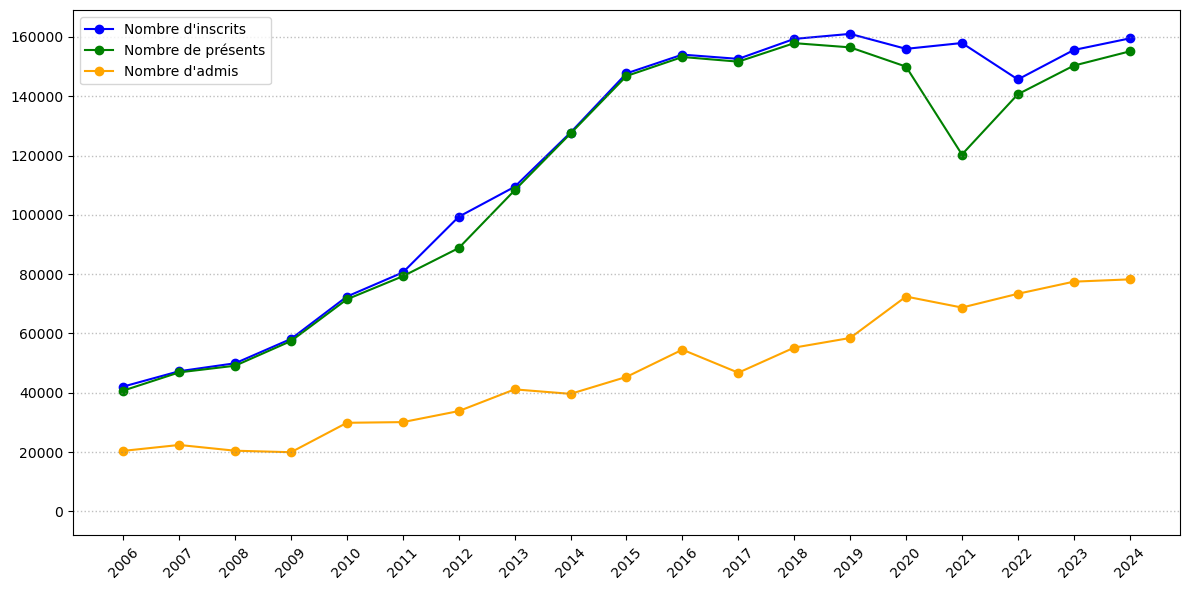
\includegraphics[width=1\textwidth]{figure/candidat.png}
\label{fig:candiadat}
\end{figure}

% \begin{figure}[h]
% \centering
% \caption{Évolution du taux de réussite au bac (2006-2024)}
% 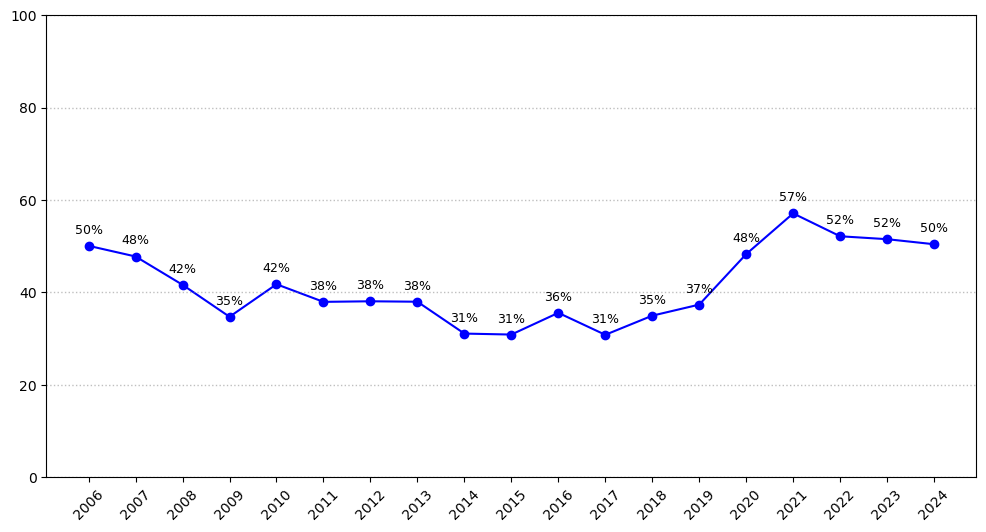
\includegraphics[width=1\textwidth]{figure/taux_de_reussite.png}
% \label{fig:taux_de_reussite}
% \end{figure}

\section{Conclusion} % Importation du chapitre 4

    \chapter{Analyse du parcours universitaire des bacheliers (UCAD)}

\section{Introduction}

\section{Analyse des résultats du baccalauréat}

\subsection{Analyse descriptive du taux de réussite}



\subsection{Étude comparative avant et après les réformes}



\subsection{Modélisation prédictive du taux de réussite}



% \section{Insertion universitaire et suivi de cohortes}

% \section{Évolution des inscriptions à l'UCAD par série du bac}



\section{Analyse du parcours universitaire des bacheliers}

\section{Conclusion} % Importation du chapitre 5

    \chapter{Restitution interactive et visualisation}

\section{Introduction}

Ce chapitre présente la phase finale de l’analyse : la restitution interactive des résultats à travers un tableau de bord conçu avec Power BI. 
L’objectif est de permettre une exploration dynamique et intuitive des données du baccalauréat sénégalais de 2006 à 2024, 
à destination notamment de l’Office du Baccalauréat et de toute personne souhaitant approfondir une étude sur le sujet.

\section{objectifs du dashboard}

Le tableau de bord a pour but :

\begin{itemize}
    \item de synthétiser les indicateurs clés liés au taux de réussite au baccalauréat par année, série et session ;
    \item d’observer l’évolution de ces indicateurs dans le temps ;
    \item de permettre un filtrage dynamique selon les besoins d’analyse ;
    \item et de soutenir la prise de décision à travers des visualisations claires et interactives.
\end{itemize}

\section{Présentation des indicateurs suivis}

Les indicateurs principaux intégrés dans le dashboard sont :
\begin{itemize}
    \item Le taux de réussite global par année ;
    \item Le taux de réussite par série ;
    \item Le nombre total d’admis et d’inscrits ;
    \item La répartition par session (1er ou 2e tour) ;
    \item La répartition par mention obtenue.
\end{itemize}

\newpage
\section{Construction du dashboard Power BI}

\subsection{Première version : Résultats de 2024 uniquement}

Dans un premier temps, n’ayant pas encore accès à l’ensemble des données historiques, 
j’ai construit une première version du tableau de bord en me basant uniquement sur les résultats de l’année 2024. 
Cette version m’a permis de tester la structure du dashboard et de définir les visualisations pertinentes à suivre. 
Elle comportait déjà tous les indicateurs énumérés précédemment.
\vspace{1cm}
\begin{figure}[htbp]
    \centering
    \caption{Tableau de bord Power BI - Résultats du baccalauréat 2024}
    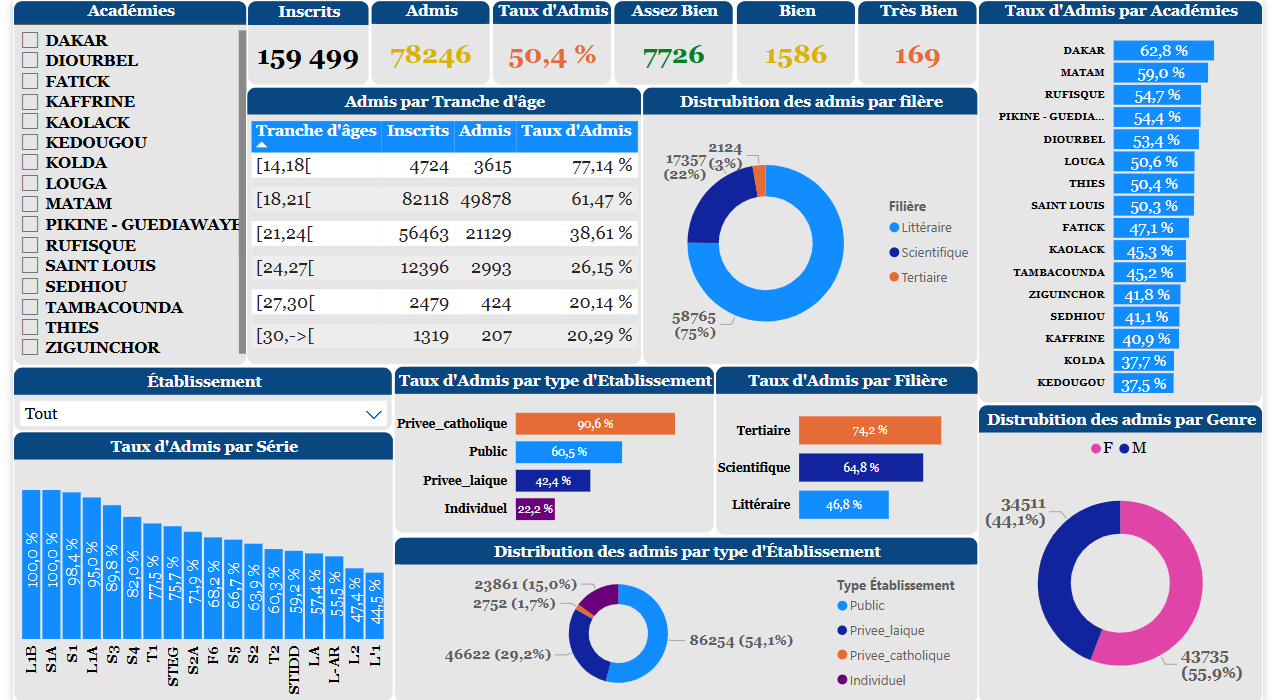
\includegraphics[width=15cm]{figure/bac_2024.png}
\end{figure}

\newpage
\subsection{ Deuxième version : Résultats de 2006 à 2024}

Une fois l’accès aux données complètes obtenu, j’ai pu enrichir le dashboard avec les résultats du bac de 2006 à 2024. 
Cette version permet d’analyser l’évolution temporelle des indicateurs clés et de mieux comprendre l’impact des différentes réformes au fil des années.
\vspace{1cm}
\begin{figure}[htbp]
    \centering
    \caption{Tableau de bord Power BI - Résultats du baccalauréat 2006 à 2024}
    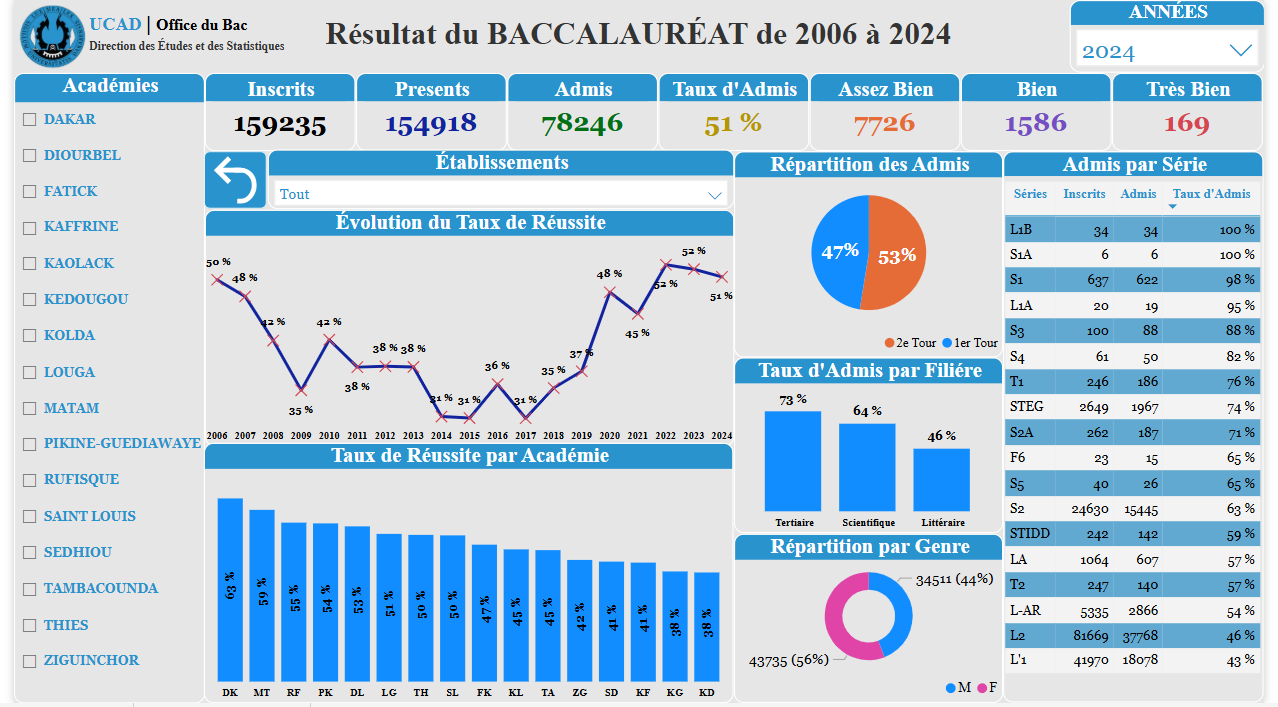
\includegraphics[width=15cm]{figure/bac_2006_2024.png}
\end{figure}

\newpage
\subsection{Utilisation de Power Query et création de mesures}

Power Query a été utilisé pour nettoyer et transformer les données importées dans Power BI. 
J’y ai notamment créé des colonnes conditionnelles pour catégoriser les mentions ou les sessions, 
et j’ai défini plusieurs mesures DAX (Data Analysis Expressions) telles que le taux de réussite, 
le nombre total d’inscrits ou encore les ratios d’admis par série.

\section{Conclusion}

La restitution interactive via Power BI offre une approche moderne et intuitive de l’analyse des données du baccalauréat. 
Elle facilite l’interprétation des tendances et appuie la prise de décision à partir d’une lecture visuelle et dynamique des résultats. 
Ce tableau de bord constitue un apport concret à l’Office du Baccalauréat, pouvant soutenir les futures études sur l’évolution du système éducatif au Sénégal. % Importation du chapitre 6
     
    \chapter*{Conclusion Générale}
\addcontentsline{toc}{chapter}{Conclusion Générale}

Ce mémoire a exploré l'impact multidimensionnel des récentes réformes du baccalauréat au Sénégal sur le taux de réussite à cet examen et sur le parcours universitaire des bacheliers à l'UCAD.

\section*{Synthèse des Contributions :}
\addcontentsline{toc}{section}{Synthèse des Contributions}

Nos principales contributions se situent à plusieurs niveaux :
\begin{enumerate}
    \item \textbf{Analyse Quantitative Approfondie :} Nous avons fourni une analyse détaillée de l'évolution des effectifs et des taux de réussite au baccalauréat sur une longue période (2006-2024), en identifiant les tendances générales et les points d'inflexion majeurs.
    \item \textbf{Impact des Réformes sur les Séries Spécifiques :} Nous avons mis en lumière le succès de la transition de la série G vers la STEG, caractérisée par une meilleure performance au bac. De même, nous avons démontré comment la réforme des filières arabes, notamment l'introduction de la série L-AR, a permis une croissance significative des effectifs et une meilleure structuration. La série S2A a également montré une dynamique positive.
    \item \textbf{Cartographie des Orientations Universitaires :} En analysant la répartition des bacheliers par établissement et département à l'UCAD, nous avons confirmé l'adéquation générale entre les séries du baccalauréat et les filières universitaires choisies, soulignant l'efficacité des réformes dans l'orientation des étudiants.
\end{enumerate}

\section*{Impact et Valeur Ajoutée :}
\addcontentsline{toc}{section}{Impact et Valeur Ajoutée}

Ce travail contribue au domaine de la Data Science appliquée à l'éducation en fournissant une analyse empirique basée sur des données réelles, ce qui est crucial pour la prise de décision politique. 
Il offre une évaluation concrète de l'efficacité des réformes éducatives, permettant aux décideurs de mieux comprendre les forces et les faiblesses du système. 
La modélisation de ces dynamiques offre des outils pour anticiper les flux d'étudiants et adapter l'offre universitaire. 
Les informations granulaires sur l'orientation peuvent aider à optimiser l'allocation des ressources dans les différents établissements et départements.

\section*{Contraintes et Limites :}
\addcontentsline{toc}{section}{Contraintes et Limites}

Il est crucial de reconnaître les contraintes rencontrées. 
L'un des défis majeurs dans l'analyse de l'impact des réformes est le facteur temps. Pour avoir une conclusion véritablement pertinente et robuste sur l'impact à long terme des réformes, notamment sur la réussite universitaire et l'insertion professionnelle, il serait nécessaire de disposer d'un recul temporel plus important. 
Les réformes les plus récentes n'ont eu que quelques années pour produire leurs effets, et l'impact complet sur le parcours universitaire (réussite en licence, master, insertion professionnelle) ne peut être pleinement mesuré qu'après plusieurs promotions complètes. 
Les données concernant les abandons ou les redoublements n'ont pas pu être intégrées en profondeur dans cette étude en raison de leur complexité et de la nécessité d'un suivi de cohorte détaillé sur plusieurs années.

\section*{Ouverture et Perspectives :}
\addcontentsline{toc}{section}{Ouverture et Perspectives}

Ce mémoire ouvre plusieurs pistes de recherche futures :
\begin{itemize}
    \item \textbf{Suivi de Cohorte Longitudinale :} Approfondir l'analyse du parcours universitaire par un suivi longitudinal des cohortes de bacheliers, en étudiant leur progression (réussite, redoublement, abandon) sur les cycles de licence et master.
    \item \textbf{Corrélation avec l'Insertion Professionnelle :} Évaluer l'adéquation entre les formations universitaires issues des nouvelles séries et les besoins du marché de l'emploi au Sénégal.
    \item \textbf{Analyse Qualitative Complémentaire :} Mener des entretiens avec les acteurs du système éducatif (enseignants, administrateurs), les bacheliers et les professionnels pour recueillir leurs perceptions des réformes.
    \item \textbf{Impact Socio-économique :} Analyser l'impact des réformes sur l'équité et l'accès à l'enseignement supérieur pour différentes catégories socio-économiques d'étudiants.
\end{itemize}


\section*{Recommandations pour les Réformes Futures :}
\addcontentsline{toc}{section}{Recommandations pour les Réformes Futures}

Au vu de cette analyse, plusieurs recommandations peuvent être formulées pour les réformes futures :
\begin{enumerate}
    \item \textbf{Consolider les Acquis des Réformes :} Poursuivre le renforcement des filières qui ont montré leur efficacité (STEG, L-AR, S2A) en assurant un alignement continu des programmes du secondaire avec les exigences de l'enseignement supérieur et du marché du travail.
    \item \textbf{Réévaluer les Filières Marginales :} Une réflexion approfondie est nécessaire concernant la série S1A et les filières S1-AR/S2-AR non implémentées. Il est essentiel de comprendre pourquoi ces filières n'attirent pas ou n'ont pas été développées, afin de les adapter, les fusionner ou les repenser si elles répondent à un besoin non satisfait.
    \item \textbf{Investir dans le Suivi des Étudiants : }Mettre en place des systèmes robustes de collecte de données longitudinales sur le parcours universitaire et l'insertion professionnelle des bacheliers. Ces données sont cruciales pour une évaluation continue et l'ajustement des politiques éducatives.
    \item \textbf{Préparer l'Université aux Nouveaux Flux :} Avec l'augmentation et la redistribution des effectifs du baccalauréat, il est impératif d'anticiper les besoins en infrastructures, en personnel enseignant et en ressources pédagogiques à l'UCAD et dans les autres établissements d'enseignement supérieur.
    \item \textbf{Communication et Orientation :} Renforcer les dispositifs d'information et d'orientation des élèves du secondaire sur les nouvelles séries du baccalauréat et les débouchés universitaires et professionnels associés, afin d'assurer des choix éclairés et une meilleure adéquation entre les profils et les filières.
\end{enumerate} % Importation du chapitre 3

    \printbibliography % Impression de la bibliographie
\end{document}